\documentclass[a4paper,12pt]{article}

\usepackage[english,russian]{babel}   
\usepackage[left=30mm, top=20mm, right=20mm, bottom=20mm, nohead, footskip=10mm]{geometry} % настройки полей документа
\usepackage[utf8]{inputenc}
\usepackage{amssymb}
\usepackage{amsfonts}
\usepackage{amsmath}
\usepackage{amsthm}
\usepackage{titlesec}
\usepackage{indentfirst}
\usepackage{graphicx}
\usepackage{cmll}
\usepackage[export]{adjustbox} % для позиционирования рисунков
\usepackage{wrapfig} % обтекание картинок текстом
\usepackage{ccaption} % подписи к рисункам

\graphicspath{{pictures/}}
\DeclareGraphicsExtensions{.png,.jpg}

\newcommand{\sectionbreak}{\clearpage}

\renewcommand{\emptyset}{\varnothing} %символ пустого множества
%\renewcommand{\bar}[1]{\overline{#1}} %растягивание всевозможных подчеркиваний
\renewcommand{\qedsymbol}{$\blacktriangleleft$} %символ QED

\theoremstyle{definition}
\newtheorem{theorem}{Теорема}[section]
\newtheorem{definition}{Определение}[section]
\newtheorem{proposal}{Утверждение}[section]

\parindent=1.25cm %отступ абзаца

\begin{document}
    \begin{titlepage}
    \begin{center}
        {\large МИНОБРНАУКИ РОССИИ
            
            ~
            
            Федеральное государственное бюджетное образовательное учреждение высшего образования
                
            «Ярославский государственный университет им. П.Г.Демидова»
            
            ~
            
            Кафедра компьютерной безопасности и
            математических методов обработки информации}
        \vfill
        
        {\large Курсовая работа}
        
        ~
        
        \textbf{{\large Алгоритм Тарского: описание и реализация}}
    \end{center}
    \vfill
    
    \newlength{\ML}
    \settowidth{\ML}{«\underline{\hspace{0.7cm}}» \underline{\hspace{2cm}}}
    \hfill\begin{minipage}{0.4\textwidth}
        Научный руководитель
        
        профессор, д-р ф.-м.н.
        \\
        \underline{\hspace{\ML}} В.\,Г.~Дурнев\\
        «\underline{\hspace{0.7cm}}» \underline{\hspace{2cm}} 2020 г.
    \end{minipage}%
    \bigskip
    
    \hfill\begin{minipage}{0.4\textwidth}
        Студент группы КБ-41СО
        \\
        \underline{\hspace{\ML}} Р.\,А.~Гибадулин\\
        «\underline{\hspace{0.7cm}}» \underline{\hspace{2cm}} 2020 г.
    \end{minipage}%
    \vfill
    
    \begin{center}
        Ярославль, 2020 г.
    \end{center}
\end{titlepage}

    \addtocounter{page}{1}

    \renewcommand*{\contentsname}{Оглавление}
\tableofcontents
    
    \section*{Введение}
	\addcontentsline{toc}{section}{Введение}

Пусть $\mathcal{A}$~--- формула логики высказываний. Задача: определить, является ли формула $\mathcal{A}$ тождественно истинной. В некотором смысле это <<трудная>> задача, однако очень просто предложить алгоритм для ее решения, но который будет <<не эффективным>>~--- алгоритм Британского музея. Рассмотрим другую задачу: определить, является ли формула \textbf{логики предикатов} тождественно истинной. Для данной задачи алгоритм перебора в общем случае уже не применим, так как множество значений переменных не обязано быть конечным. Но оказывается, для некоторых языков логики предикатов существуют алгоритмы решающие эту задачу. Одним из таких алгоритмов и является алгоритм Тарского, описанию и реализации которого посвящена данная работа.

\textbf{Цели работы:} изучить и описать алгоритм Тарского, и реализовать его в виде компьютерной программы.

\textbf{Задачи:}
\begin{itemize}
	\item Ввести определения, сформулировать и доказать утверждения необходимые для описания алгоритма Тарского;
	\item Реализовать компьютерную программу, которая по формуле элементарной алгебры без параметров   введенной с клавиатуры, строит эквивалентную бескванторную формулу того же языка. 
\end{itemize}

В первой части данной работы будет определен язык элементарной алгебры, дано определение элиминации кванторов и сформулировано утверждения о ней. Далее пойдет речь об идеях, на которых основан алгоритм, будут определены таблицы Тарского. Затем будут даны определения полунасыщенной и насыщенной систем многочленов, после чего будет описан метод построения таблиц Тарского, что практически завершит описание алгоритма Тарского.

Во второй части подробно рассматривается программа, написанная и отлаженная автором работы, а именно описано как происходит распознавание формулы, какие при этом используются алгоритмы, как организованно представление формул, описываются реализации насыщения системы многочленов и построения таблицы Тарского. 





    \section{Алгоритм Тарского}

Прежде всего определим область математики, истинность утверждений которой должен проверять алгоритм. Затем формально опишем язык, на котором записываются эти утверждения. И, наконец, опишем алгоритм, который по формуле описанного языка строит эквивалентную бескванторную формулу.

\subsection{Элементарная алгебра}

Под элементарной алгеброй понимается та часть общей теории действительных чисел, в которой используются переменные, представляющие собой действительные числа, и константы для всех рациональных чисел, определены арифметические операции, такие как <<сложение>> и <<умножение>>, и отношения сравнения действительных чисел~--- <<меньше>>, <<больше>> и <<равно>>. То есть рассматриваются системы алгебраических уравнений и неравенств.

Заметим, что используя декартову систему координат, некоторые задачи геометрии можно сформулировать как задачи элементарной алгебры. Например, теорема о пересечении высот треугольника, которая утверждает, что три высоты невырожденного треугольника пересекаются в одной точке, равносильна утверждению: для любых трех точек $A(x_1, y_1)$, $B(x_2, y_2)$ и $C(x_3, y_3)$, не лежащих на одной прямой, существует точка $D(x_4, y_4)$ такая, что $\overrightarrow{AD} \perp \overrightarrow{BC}$, $\overrightarrow{BD} \perp \overrightarrow{AC}$ и $\overrightarrow{CD} \perp \overrightarrow{AB}$. Иначе говоря, если $\overrightarrow{AB} \land \overrightarrow{AC} \neq 0$, то система
\begin{equation*}
    \begin{cases}
        \left(\overrightarrow{AD}, \overrightarrow{BC}\right) = 0 \\
        \left(\overrightarrow{BD}, \overrightarrow{AC}\right) = 0 \\
        \left(\overrightarrow{CD}, \overrightarrow{AB}\right) = 0
    \end{cases}
\end{equation*}
имеет решение относительно переменных $x_4$, $y_4$, где $* \land *$~--- псевдоскалярное произведение векторов, $(*, *)$~--- скалярное произведение векторов.

\subsection{Язык элементарной алгебры}

Язык элементарной алгебры~--- это язык логики первого порядка с сигнатурой
\begin{equation*}
    \tau = \langle \, \mathbb{Q},\, F,\, P,\, \theta,\, \phi \, \rangle,
\end{equation*}
где $\mathbb{Q}$~--- множество рациональных чисел, которое является множеством индивидных констант, $F =  \left\{+,\, \cdot\right\}$~--- множество функциональных символов, $P = \left\{ <,\, >,\, = \right\}$~--- множество предикатных символов, $\theta : F \rightarrow \mathbb{N}$ такое, что $\theta(+) = 2$ и $\theta(\cdot) = 2$, и $\phi : P \rightarrow \mathbb{N}$ такое, что $\phi(<) = 2$, $\phi(>) = 2$ и $\phi(=) = 2$. Из определения отображений $\theta$ и $\phi$ следует, что все $f \in F$ являются двухместными функциональными символами, а все $p \in P$ являются двухместными предикатными символами. Основное множество интерпретации языка $L_\tau $ совпадает с множеством действительных чисел $\mathbb{R}$, отображение множества индивидных констант в основное множество определяется естественным образом, так как $\mathbb{Q} \subset \mathbb{R}$, функциональные символы $+$ и $\cdot$ отображаются в сложение и умножение в поле $\mathbb{R}$ соответственно, и предикатные символы $<$, $>$ и $=$ отображаются естественным образом в операции сравнения в $\mathbb{R}$.

%\begin{remark}
    Множество констант ограничено рациональными числами лишь потому, что компьютер может быстро работать с ними без потери точности, что нельзя сказать про действительные числа.
%\end{remark}

Например, теорема о пересечении высот на языке элементарной алгебры записывается так:
\begin{gather*}
    (\forall x_1)(\forall y_1)(\forall x_2)(\forall y_2)(\forall x_3)(\forall y_3) \\
    (
        (
            \lnot
            (
                (x_2 - x_1)\cdot(y_3 - y_1) - (y_2 - y_1)\cdot(x_3 - x_1) = 0
            )
        )
        \to \\
        (\exists x_4)(\exists y_4)
        (
           (
                (x_4 - x_3)\cdot(x_2 - x_1) + (y_4 - y_3)\cdot(y_2 - y_1) = 0
            ) \& \\
            (
                (x_4 - x_2)\cdot(x_1 - x_3) + (y_4 - y_2)\cdot(y_1 - y_3) = 0
            ) \& \\
            (
                (x_4 - x_1)\cdot(x_3 - x_2) + (y_4 - y_1)\cdot(y_3 - y_2) = 0
            )
        )
    ).
\end{gather*}

%\begin{remark}
    Нет необходимости формально вводить такие операции как вычитание, деление и возведение в степень по следующим соображениям:
    \begin{equation*}
        a-b=a+(-1)\cdot b; \quad \frac{a}{b} > 0 \Leftrightarrow (a > 0 \, \& \, b > 0) \lor (a < 0 \, \& \, b < 0); \quad x^2 = x \cdot x.
    \end{equation*}
%\end{remark}

\subsection{Элиминация кванторов}

\begin{definition}
    \textbf{Элиминация кванторов}~--- это процесс, порождающий по заданной логической формуле, другую, эквивалентную ей бескванторную формулу, то есть свободную от вхождений кванторов.
\end{definition}

Пусть алгоритм $A$ такой, что $A\left(\left(Qx\right)\mathcal{A}\right) = \mathcal{B}$, где $\mathcal{A}$ и $\mathcal{B}$~--- бескванторные формулы языка элементарной алгебры, и формулы $(Qx)\mathcal{A}$ и $\mathcal{B}$ эквивалентны, а $Q$~--- квантор. Тогда верно следующее утверждение:
\begin{proposal}\label{algB}
    Если алгоритм $A$ существует, то существует алгоритм $B$ такой, что для любой формулы $\mathcal{A}$ языка элементарной алгебры $B\left(\mathcal{A}\right)$~--- бескванторная формула, эквивалентная $\mathcal{A}$.
\end{proposal}   
\begin{proof}
    Определим алгоритм $B$ следующим образом:
    \begin{itemize}
        \item Если $\mathcal{A}$~--- бескванторная формула, то $B\left(\mathcal{A}\right) = \mathcal{A}$;
        \item Если $\mathcal{A} = \left(Qx\right)\mathcal{B}$, то $B\left(\mathcal{A}\right) = A\left(\left(Qx\right)B\left(\mathcal{B}\right)\right)$. Формула $B\left(\mathcal{B}\right)$~--- бескванторная по построению $B$, следовательно запись $A\left(\left(Qx\right)B\left(\mathcal{B}\right)\right)$ корректна, при этом $B\left(\mathcal{B}\right)$ эквивалентна $\mathcal{B}$, следовательно, $\left(Qx\right)\mathcal{B}$ эквивалентна $\left(Qx\right)B\left(\mathcal{B}\right)$, а значит $\mathcal{A}$ эквивалентна $B\left(\mathcal{A}\right)$. Также заметим, что длина формулы $\mathcal{B}$ строго меньше длины формулы $\mathcal{A}$;
        \item Если $\mathcal{A}$ не удовлетворяет предыдущим условиям, то
        \begin{itemize}
            \item либо $\mathcal{A} = \lnot \mathcal{B}$, тогда $B\left(\mathcal{A}\right) = \lnot B\left(\mathcal{B}\right)$,
            \item либо $\mathcal{A} = \mathcal{B} * \mathcal{C}$, тогда $B\left(\mathcal{A}\right) = B\left(\mathcal{B}\right) * B\left(\mathcal{C}\right)$, где $* \in \left\{\lor, \&, \to\right\}$.
        \end{itemize}
        При этом длины формул $\mathcal{B}$ и $\mathcal{C}$ меньше длины формулы $\mathcal{A}$.
    \end{itemize}
    Алгоритм $B$ определен рекурсивно, при этом на каждом этапе на вход $B$ подаётся формула меньшей длины, следовательно, алгоритм $B$ является конечным, и на каждом шаге выход алгоритма~--- бескванторная эквивалентная формула.
\end{proof} 
%\begin{remark}
    Данное утверждение верно и для других языков логики предикатов.
%\end{remark}

Таким образом, для элиминации кванторов произвольной формулы достаточно построить алгоритм $A$ и применить описанный в утверждении \ref{algB} алгоритм $B$.

\subsection{Алгоритм Тарского}

Термы в языке элементарной алгебры~--- это многочлены с рациональными коэффициентами от действительных переменных Тогда очевидно, что выражения
\begin{equation*}
    f < g, \quad f = g, \quad f > g
\end{equation*}
равносильны выражениям
\begin{equation*}
    f - g < 0, \quad f - g = 0, \quad f - g > 0 
\end{equation*}
соответственно, где $f$ и $g$~--- термы. Поэтому, не нарушая общности рассуждений, можно считать, что все атомарные формулы имеют вид:
\begin{equation*}
    f < 0, \quad f = 0, \quad f > 0.
\end{equation*}
Поэтому нас будет интересовать только знак многочлена.

%\begin{remark}
    На данном этапе можно считать, что все рассматриваемые многочлены ненулевые, так как знак нулевого многочлена в любой точке определяется тривиальным образом.
%\end{remark}

Рассмотрим формулу $\mathcal{A} = (Qx)(f(x) \, \rho \, 0)$, где $Q$~--- квантор, $f(x)$~--- многочлен от одной переменной, $\rho$~--- предикат. Известно, что многочлены от одной переменной сохраняют свой знак, то есть на интервалах между корнями значение предиката неравенства или равенства с нулем постоянно. Следовательно, чтобы уметь определять знак значения многочлена в произвольной точке, достаточно знать значения многочлена лишь в \textbf{конечном} наборе точек~--- во всех корнях, в каких-то точках между любой парой соседних корней, а также в точках, одна из которых заведомо правее, а другая~--- левее всех корней. Тогда формуле $\mathcal{A}$ эквивалентна следующая бескванторная формула:
\begin{equation*}
    \mathcal{B} = 
    \begin{cases}
        \bigvee\limits_{x_0 \in X} (f(x_0) \, \rho \, 0), &\text{если $Q = \exists$} \\
        \bigwith\limits_{x_0 \in X} (f(x_0) \, \rho \, 0), &\text{если $Q = \forall$} \\
    \end{cases}
\end{equation*}
где $X$~--- конечное множество этих точек.

Рассмотрим формулу $\mathcal{A} = (Qx)(\Phi(x))$, где $\Phi(x)$~--- бескванторная формула, которая может содержать вхождения лишь переменной $x$. Аналогично предыдущему случаю, пусть множество $X$ состоит из корней многочленов, входящих в формулу $\Phi(x)$, и точек, выбранных между парами соседних корней, а также пусть в это множество входит точка, которая правее всех корней, и точка, которая левее всех корней. Тогда формула
\begin{equation*}
    \mathcal{B} = 
    \begin{cases}
        \bigvee\limits_{x_0 \in X} \Phi(x_0), &\text{если $Q = \exists$} \\
        \bigwith\limits_{x_0 \in X} \Phi(x_0), &\text{если $Q = \forall$} \\
    \end{cases}
\end{equation*}
свободна от вхождений кванторов и эквивалента формуле $\mathcal{A}$.

По теореме Ролля о нуле производной, для любой пары корней $x_1, x_2$ между ними существует такая точка $\xi$, что производная многочлена в точке $\xi$ обращается в ноль. Поэтому в качестве точек между корнями можно использовать корни производной этого многочлена.

Аналогично, множество корней многочлена
\begin{equation*}
    \prod\limits_{i = 1}^n f_i(x)
\end{equation*}
совпадает с объединением множеств корней многочленов $f_1(x), ... , f_n(x)$, тогда в качестве точек между корнями можно рассматривать корни многочлена
\begin{equation*}
    f_0(x) = \left(\prod\limits_{i = 1}^n f_i(x)\right)^\prime. 
\end{equation*}

\subsubsection{Таблица Тарского}

Упорядочим выбранные точки $X = \left\{x_1, ... , x_s\right\}$ по возрастанию и запишем значения многочленов в этих точках в таблицу:
\begin{center}
    \begin{tabular}{ |c|c|c|c|c|c| } 
    \hline
                 & $x_1$ & $...$ & $x_j$ & $...$ & $x_s$ \\ 
    \hline
        $f_1$ & $f_1(x_1)$ & $...$ & $f_1(x_j)$ & $...$ & $f_1(x_s)$\\ 
    \hline
        $\vdots$ & $\vdots$ & $\ddots$ & $\vdots$ & $\ddots$ & $\vdots$ \\
    \hline
        $f_i$ & $f_i(x_1)$ & $...$ & $f_i(x_j)$ & $...$ & $f_i(x_s)$\\ 
    \hline
        $\vdots$ & $\vdots$ & $\ddots$ & $\vdots$ & $\ddots$ & $\vdots$ \\
    \hline
        $f_n$ & $f_n(x_1)$ & $...$ & $f_n(x_j)$ & $...$ & $f_n(x_s)$\\    
    \hline
    \end{tabular}
\end{center}
Так как нас интересуют только знаки многочленов в этих точках, то достаточно записывать лишь символ знака значения:
\begin{center}
    \begin{tabular}{ |c|c|c|c|c|c| } 
    \hline
                 & $x_1$ & $...$ & $x_j$ & $...$ & $x_s$ \\ 
    \hline
        $f_1$ & $\varepsilon_{11}$ & $...$ & $\varepsilon_{1j}$ & $...$ & $\varepsilon_{1s}$\\ 
    \hline
        $\vdots$ & $\vdots$ & $\ddots$ & $\vdots$ & $\ddots$ & $\vdots$ \\
    \hline
        $f_i$ & $\varepsilon_{i1}$ & $...$ & $\varepsilon_{ij}$ & $...$ & $\varepsilon_{is}$\\ 
    \hline
        $\vdots$ & $\vdots$ & $\ddots$ & $\vdots$ & $\ddots$ & $\vdots$ \\
    \hline
        $f_n$ & $\varepsilon_{n1}$ & $...$ & $\varepsilon_{nj}$ & $...$ & $\varepsilon_{ns}$\\    
    \hline
    \end{tabular}
\end{center}
где 
\begin{equation*}
    \varepsilon_{ij} = 
    \begin{cases}
        +, &\text{если $f_i(x_j) > 0$} \\
        0, &\text{если $f_i(x_j) = 0$} \\
        -, &\text{если $f_i(x_j) < 0$}
    \end{cases}.
\end{equation*}
Таблицы такого вида будем называть \textbf{таблицами Тарского}. 

\begin{proposal}
    Знаки $+$ и $-$ не могут стоять в двух соседних по горизонтали клетках таблицы Тарского.
\end{proposal}
\begin{proof}
    Следует из теоремы Коши о нулях непрерывной функции, непрерывности многочленов как функций и упорядоченности точек $x_1, ..., x_s$.
\end{proof}

Имея таблицу Тарского, нетрудно вычислить истинностное значение формулы $\Phi(x_i)$, так как для определения истинностного значения атомарной формулы достаточно посмотреть на соответствующую клетку таблицы. При этом уже нет необходимости знать точки $x_1, ..., x_n$. А зная истинностное значение формулы, можно построить эквивалентную бескванторную:
\begin{itemize}
    \item если формула истинна~--- то можно использовать любую тождественно истинную формулу, например, $0=0$;
    \item если формула ложна~--- то можно использовать любую тождественно ложную формулу, например $0=1$.
\end{itemize}

До сих пор не обсуждалось, как искать корни многочленов. Оказывается, таблицу Тарского можно построить не находя ни одного корня, если рассмотреть системы многочленов особого вида.

\subsubsection{Насыщенная система}

\begin{definition}\cite{lect1}
    Система функций называется \textbf{полунасыщенной}, если вместе с каждой функцией, отличной от постоянной функции, она содержит и ее производную.
\end{definition}

\begin{proposal}\cite{lect1}
    Каждую конечную систему многочленов можно расширить до конечной полунасыщенной системы.
\end{proposal}

\begin{proposal}\label{two zero}\cite{lect1}
    Если многочлен отличен от тождественного нуля, то в строке таблицы Тарского, соответствующей этому многочлену, в соседних по горизонтали клетках не могут стоять два символа 0.
\end{proposal}

\begin{definition}\cite{lect1}
    Полунасыщенная система многочленов $p_1(x), ... , p_n(x)$ называется \textbf{насыщенной}, если вместе с каждыми двумя многочленами $p_i(x)$ и $p_j(x)$ такими, что $0 < deg(p_j(x)) \leq deg(p_i(x))$, она содержит и остаток $r(x)$ от деления $p_i(x)$ на $p_j(x)$. 
\end{definition}

\begin{proposal}\cite{lect1}
    Каждую конечную систему многочленов можно расширить до конечной насыщенной системы.
\end{proposal}

\begin{proposal}\label{subsystem}\cite{lect1}
    Если $p_1(x), ... , p_{n-1}(x), p_n(x)$~--- насыщенная система многочленов, и 
    \begin{equation*}
        deg(p_1(x)) \leq ... \leq deg(p_{n-1}(x)) \leq deg(p_n(x)),
    \end{equation*}
    то система $p_1(x), ... , p_{n-1}(x)$ также является насыщенной.
\end{proposal}

\begin{proposal}\label{min deg}
    Если $p_1(x), ... , p_n(x)$~--- насыщенная система многочленов, и 
    \begin{equation*}
        deg(p_1(x)) \leq deg(p_i(x)),\,\text{где $i = 2, 3, ... , n$},
    \end{equation*}
    то $deg(p_1(x)) < 1$.
\end{proposal}
\begin{proof}
    Если предположить противное, то с одной стороны, система должна содержать многочлен $p_1^\prime(x)$, степень которого меньше $deg(p_1(x))$, а с другой стороны, степени всех многочленов должны быть не меньше $deg(p_1(x))$, противоречие.
\end{proof}

\subsubsection{Метод построения таблицы Тарского}

Пусть $p_1(x), ... , p_{n-1}(x), p_n(x)$~--- насыщенная система многочленов, и многочлены упорядочены в ней по не убыванию степени.

Рассмотрим подсистему из одного элемента $p_1(x)$. Согласно утверждению \ref{subsystem}, система $p_1(x)$ является насыщенной, тогда многочлен $p_1(x)$ представляет собой константу, так как его степень меньше единицы, согласно утверждению \ref{min deg}. В таком случае знак многочлена в любой точке совпадает со знаком этой константы. Таблица Тарского для одного многочлена имеет вид:
\begin{center}
    \begin{tabular}{ |c|c|c| } 
    \hline
        & $-\infty$ & $+\infty$ \\ 
    \hline
        $p_1$ & $\varepsilon$ & $\varepsilon$\\ 
    \hline
    \end{tabular}
\end{center}
Символами $-\infty$ и $+\infty$ обозначены точки, которые заведомо расположены левее и правее всех корней соответственно. Выбирать конкретные значения для этих точек не нужно, потому что в точке $+\infty$ знак многочлена совпадает со знаком старшего коэффициента, а в точке $-\infty$ знак зависит от четности степени многочлена:
\begin{itemize}
    \item если четная, то совпадает со знаком старшего коэффициента;
    \item иначе равен знаку противоположному к знаку старшего коэффициента.
\end{itemize}
В таблице всего два столбца, поэтому верно утверждение: для каждого столбца $j$, за исключением самого правого и самого левого, в этой таблице существует ненулевой многочлен $p_i(x)$ такой, что $\varepsilon_{i, j} = 0$.

Индуктивное предположение: пусть для насыщенной системы $p_1(x), ... , p_{k-1}(x)$ уже построена таблица Тарского:
\begin{center}
    \begin{tabular}{ |c|c|c|c|c|c| } 
    \hline
                 & $-\infty$ & $...$ &  & $...$ & $+\infty$ \\ 
    \hline
        $p_1$ & $\varepsilon_{1, 1}$ & $...$ & $\varepsilon_{1, j}$ & $...$ & $\varepsilon_{1, s}$\\ 
    \hline
        $\vdots$ & $\vdots$ & $\ddots$ & $\vdots$ & $\ddots$ & $\vdots$ \\
    \hline
        $p_{k-1}$ & $\varepsilon_{k-1, 1}$ & $...$ & $\varepsilon_{k-1, j}$ & $...$ & $\varepsilon_{k-1, s}$\\    
    \hline
    \end{tabular}
\end{center}
И для каждого столбца $j$, за исключением самого правого и самого левого, в этой таблице существует ненулевой многочлен $p_i(x)$ такой, что $\varepsilon_{i, j} = 0$.

К этой таблице добавим строку для многочлена $p_{k}(x)$, записав знаки для крайних столбцов.
\begin{center}
    \begin{tabular}{ |c|c|c|c|c|c| } 
    \hline
                 & $-\infty$ & $...$ &  & $...$ & $+\infty$ \\ 
    \hline
        $p_1$ & $\varepsilon_{1, 1}$ & $...$ & $\varepsilon_{1, j}$ & $...$ & $\varepsilon_{1, s}$\\ 
    \hline
        $\vdots$ & $\vdots$ & $\ddots$ & $\vdots$ & $\ddots$ & $\vdots$ \\
    \hline
        $p_{k-1}$ & $\varepsilon_{k-1, 1}$ & $...$ & $\varepsilon_{k-1, j}$ & $...$ & $\varepsilon_{k-1, s}$\\    
    \hline
        $p_{k}$ & $\varepsilon_{k, 1}$ & $...$ & $ $?$ $ & $...$ & $\varepsilon_{k, s}$\\    
    \hline
    \end{tabular}
\end{center}
Для каждого столбца $j$ рассмотрим многочлен $p_i(x)$ такой, что $\varepsilon_{i, j} = 0$. Этот многочлен существует и отличен от тождественного нуля в силу индуктивного предположения.
\begin{proposal}\label{остаток}
    Пусть $f(x)$ и $g(x)$~--- ненулевые многочлены. Если $g(a) = 0$, то f(a) = r(a), где r(x)~--- остаток от деления многочлена f(x) на g(x).
\end{proposal}
\begin{proof}
    Многочлен $r(x)$~--- остаток от деления, тогда $f(x) = q(x)g(x) + r(x)$, подставив $a$ получим $f(a) = q(a)g(a) + r(a) = q(a)\cdot 0 + r(a) = r(a)$.
\end{proof}

Найдём $p_t(x)$~--- остаток от деления $p_k(x)$ на $p_i(x)$. Система многочленов насыщена, поэтому многочлен $p_t(x)$ уже добавлен в таблицу, следовательно, по утверждению \ref{остаток}, $\varepsilon_{k, j} = \varepsilon_{t, j}$. Таким образом, заполняется вся нижняя строка.

Просмотрим значения в нижней строке. Может случиться так, что в соседних клетках стоят знаки $+$ и $-$. В таком случае необходимо добавить новый столбец между теми столбцами, в которых находятся эти клетки. Понятно, что в новом столбце нижняя клетка заполняется нулем, что следует из теоремы Коши о нулях непрерывной функции. Для оставшихся клеток рассмотрим случаи.
\begin{center}
    \begin{tabular}{|c|c|c|}
        \hline
        $+$ & ? & $+$\\
        \hline
    \end{tabular}
        \quad
    \begin{tabular}{|c|c|c|}
        \hline
        $+$ & ? & $0$\\
        \hline
    \end{tabular}           
\end{center}
Тогда вместо символа $?$ ставится знак $+$.
\begin{center}
    \begin{tabular}{|c|c|c|}
        \hline
        $0$ & ? & $+$\\
        \hline
    \end{tabular}
        \quad
    \begin{tabular}{|c|c|c|}
        \hline
        $0$ & ? & $-$\\
        \hline
    \end{tabular}           
\end{center}
В этих случаях ставится знак $+$ или $-$ соответственно.
\begin{center}
    \begin{tabular}{|c|c|c|}
        \hline
        $-$ & ? & $0$\\
        \hline
    \end{tabular}
        \quad
    \begin{tabular}{|c|c|c|}
        \hline
        $-$ & ? & $-$\\
        \hline
    \end{tabular}           
\end{center}
В этих~--- знак $-$.
И наконец, в случае 
\begin{center}
    \begin{tabular}{|c|c|c|}
        \hline
        $0$ & ? & $0$\\
        \hline
    \end{tabular} 
\end{center}
ставится $0$, так как эта строка точно соответствует нулевому многочлену.

А случаи
\begin{center}
    \begin{tabular}{|c|c|c|}
        \hline
        $+$ & ? & $-$\\
        \hline
    \end{tabular}
        \quad
    \begin{tabular}{|c|c|c|}
        \hline
        $-$ & ? & $+$\\
        \hline
    \end{tabular}      
\end{center}
невозможны по построению таблицы Тарского.

Таким образом, удалось построить таблицу Тарского для насыщенной системы многочленов $p_1(x), ... , p_{k-1}(x), p_k(x)$, при этом для каждого столбца найдется многочлен, на пересечении строки которого с выбранным столбцом в клетке записан символ $0$.

\subsubsection{Алгоритм для формулы вида $(Qx)\Phi(x)$}

Все готово, чтобы описать алгоритм Тарского для формулы $\mathcal{A} = (Qx)\Phi(x)$:
\begin{enumerate}
    \item Составить список всех многочленов $f_1(x), ... , f_n(x)$, входящих в $\Phi(x)$ и отличных от тождественного нуля;
    \item Добавить к этому списку многочлен 
    \begin{equation*}
        f_0(x) = \left( \prod\limits_{i = 1}^n f_i(x) \right)^\prime;
    \end{equation*}
    \item Расширить этот список до насыщенной системы $p_1(x), ... , p_m(x)$, упорядоченной по не убыванию степени;
    \item Построить таблицу Тарского, по очереди добавляя многочлены; 
    \item Вычислить истинностное значение $\Phi(x)$ для каждого из столбцов таблицы;
    \item Если $Q = \exists$, то формула $\mathcal{A}$ истинна тогда и только тогда, когда хотя бы одно из вычисленных значений истинно. Если $Q = \forall$, то формула $\mathcal{A}$ истинна тогда и только тогда, когда все вычисленные значения истинны.
\end{enumerate}

\subsubsection{Алгоритм для формулы вида $(Qx)\Phi(x, a_1, ... , a_l)$}

Оказывается, в случае, когда формула имеет вид $(Qx)\Phi(x, a_1, ... , a_l)$, нужно лишь немного модифицировать алгоритм. Во-первых, коэффициенты многочленов теперь не из $\mathbb{Q}$, а из поля частных целостного кольца $\mathbb{Q}\left[a_1, ... , a_l\right]$. Во-вторых, нельзя говорить о знаках таких коэффициентов, поэтому каждый раз, когда необходимо определить знак коэффициента, придется разбирать три случая: коэффициент меньше нуля, больше нуля или равен нулю. Поэтому будет построено дерево разбора случаев. В листьях этого дерева все знаки определены и можно построить таблицу Тарского. Если по таблице получается, что формула истинна, тогда все предположения, сделанные в ходе разбора случаев, выписываются в виде конъюнкции. Результатом же работы алгоритма будет дизъюнкция всех таких конъюнкций.

\subsubsection{Пример работы алгоритма}
Рассмотрим формулу $(\forall x)(y < 0 \, \to \, x^2 > y)$ и построим эквивалентную ей бескванторную формулу с помощью алгоритма Тарского. Многочлены $y$ и $x^2 - y$ входят в данную формулу. Далее нужно выяснить все ли многочлены отличны от тождественного нуля, поэтому рассмотрим два случая:
\begin{enumerate}
    \item $y = 0$, тогда из списка исключается многочлен $y \equiv 0$ и добавляется многочлен $2x$, при этом $x^2 - y \equiv x^2$;
    \item $y < 0$ или $y > 0$, тогда в систему добавляется многочлен $2yx$.
\end{enumerate}
Переходим к насыщению системы:
\begin{enumerate}
    \item система $2x, x^2$ дополняется до $0, 2, 2x, x^2$;
    \item система $y, 2yx, x^2 - y$ дополняется до $0, y, -y, 2y, 2, 2yx, 2x, x^2 - y$.
\end{enumerate}
Построим таблицы Тарского:
\begin{enumerate}
    \item $y = 0$, система $0, 2, 2x, x^2$:
    \begin{center}
        \begin{tabular}{|c|c|c|}
            \hline
             & $-\infty$ & $+\infty$\\
            \hline
            $0$ & $0$ & $0$\\
            \hline
            $2$ & $+$ & $+$\\
            \hline
        \end{tabular} 
            \quad
        \begin{tabular}{|c|c|c|c|}
            \hline
             & $-\infty$ & & $+\infty$\\
            \hline
            $0$ & $0$ & $0$ & $0$\\
            \hline
            $2$ & $+$ & $+$ & $+$\\
            \hline
            $2x$ & $-$ & $0$ & $+$\\
            \hline
        \end{tabular}
            \quad
        \begin{tabular}{|c|c|c|c|}
            \hline
             & $-\infty$ & & $+\infty$\\
            \hline
            $0$ & $0$ & $0$ & $0$\\
            \hline
            $2$ & $+$ & $+$ & $+$\\
            \hline
            $2x$ & $-$ & $0$ & $+$\\
            \hline
            $x^2$ & $+$ & $0$ & $+$\\
            \hline
        \end{tabular}         
    \end{center}
    \item $y < 0$, система $0, y, -y, 2y, 2, 2yx, 2x, x^2 - y$:
    \begin{center}
        \begin{tabular}{|c|c|c|}
            \hline
             & $-\infty$ & $+\infty$\\
            \hline
            $0$ & $0$ & $0$\\
            \hline
            $y$ & $-$ & $-$\\
            \hline
            $-y$ & $+$ & $+$\\
            \hline
            $2y$ & $-$ & $-$\\
            \hline
            $2$ & $+$ & $+$\\
            \hline
        \end{tabular} 
            \quad
        \begin{tabular}{|c|c|c|c|}
            \hline
             & $-\infty$ & & $+\infty$\\
            \hline
            $0$ & $0$ & $0$ & $0$\\
            \hline
            $y$ & $-$ & $-$ & $-$\\
            \hline
            $-y$ & $+$ & $+$ & $+$\\
            \hline
            $2y$ & $-$ & $-$ & $-$\\
            \hline
            $2$ & $+$ & $+$ & $+$\\
            \hline
            $2yx$ & $+$ & $0$ & $-$\\
            \hline
            $2x$ & $-$ & $0$ & $+$\\
            \hline
            $x^2 - y$ & $+$ & $+$ & $+$\\
            \hline
        \end{tabular} 
            \quad    
    \end{center}
    \item $y > 0$, система $0, y, -y, 2y, 2, 2yx, 2x, x^2 - y$:
    \begin{center}
        \begin{tabular}{|c|c|c|}
            \hline
             & $-\infty$ & $+\infty$\\
            \hline
            $0$ & $0$ & $0$\\
            \hline
            $y$ & $+$ & $+$\\
            \hline
            $-y$ & $-$ & $-$\\
            \hline
            $2y$ & $+$ & $+$\\
            \hline
            $2$ & $+$ & $+$\\
            \hline
        \end{tabular} 
            \quad
        \begin{tabular}{|c|c|c|c|}
            \hline
             & $-\infty$ & & $+\infty$\\
            \hline
            $0$ & $0$ & $0$ & $0$\\
            \hline
            $y$ & $+$ & $+$ & $+$\\
            \hline
            $-y$ & $-$ & $-$ & $-$\\
            \hline
            $2y$ & $+$ & $+$ & $+$\\
            \hline
            $2$ & $+$ & $+$ & $+$\\
            \hline
            $2yx$ & $-$ & $0$ & $+$\\
            \hline
            $2x$ & $-$ & $0$ & $+$\\
            \hline
        \end{tabular} 
            \quad 
        \begin{tabular}{|c|c|c|c|c|c|}
            \hline
             & $-\infty$ & & & & $+\infty$\\
            \hline
            $0$ & $0$ & $0$ & $0$ & $0$ & $0$\\
            \hline
            $y$ & $+$ & $+$ & $+$ & $+$ & $+$\\
            \hline
            $-y$ & $-$ & $-$ & $-$ & $-$ & $-$\\
            \hline
            $2y$ & $+$ & $+$ & $+$ & $+$ & $+$\\
            \hline
            $2$ & $+$ & $+$ & $+$ & $+$ & $+$\\
            \hline
            $2yx$ & $-$ & $-$ & $0$ & $+$ & $+$\\
            \hline
            $2x$ & $-$ & $-$ & $0$ & $+$ & $+$\\
            \hline
            $x^2 - y$ & $+$ & $0$ & $-$ & $0$ & $+$\\
            \hline
        \end{tabular} 
            \quad       
    \end{center}
\end{enumerate}
Нетрудно убедиться в том, что для каждого случая, для каждого столбца формула $(y < 0 \, \to \, x^2 > y)$ истинна. В результате, на выходе алгоритма получим формулу
\begin{equation*}
    (y = 0 \lor y < 0 \lor y > 0).
\end{equation*}

\subsection{Теорема Тарского}

\begin{theorem}[Альфред Тарский]
    Для любой формулы $\mathcal{A}$ языка элементарной алгебры существует эквивалентная ей бескванторная формула этого же языка.
\end{theorem}


Алгоритм, предложенный А. Тарским в его работе \cite{Tarski}, записывался иначе~--- предельно формально. Но и цель была не предложить <<хороший>> алгоритм, а доказать, что элементарная алгебра допускает элиминацию кванторов. В последующие годы велась работа по упрощению и усовершенствованию алгоритма, особенно в случае вхождений свободных переменных, и в результате этой работы алгоритм приобрел такой вид. Современное, менее формальное описание алгоритма доступнее для понимания, что, например, упрощает реализацию алгоритма.

    \section{Программная реализация}

После изучения алгоритма Тарского была начата работа по реализации этого алгоритма, но не для произвольных формул, а для формул без параметров.

\begin{definition}
    Формула $\mathcal{A}$ называется \textbf{формулой без параметров}, если для любой ее подформулы вида $(Qx)\mathcal{B}$, формула $\mathcal{B}$ свободна от вхождений кванторов и от переменных, возможно, за исключением переменной $x$.
\end{definition}

Для этого были выбраны язык C\#, платформа .NET Core 3.1 и спецификация .NET Standard 2.1 \cite{TroelsonNet}. Такой выбор обусловлен рядом причин:
\begin{itemize}
    \item Язык C\#~--- это объектно-ориентированный язык программирования, а данная парадигма программирования позволяет абстрактно описывать объекты, в том числе и математические объекты; 
    \item .NET Core и .NET Standard~--- это современные, развивающиеся и востребованные кроссплатформенные технологии с открытым исходным кодом;
    \item Личные предпочтения автора.
\end{itemize}
Для поэтапного создания программы, были сформулированы и решены следующие задачи:
\begin{itemize}
    \item Разработать библиотеку классов для объектов языка элементарной алгебры: символы алфавита, термы, формулы;
    \item Реализовать ввод логических формул, то есть решить задачу лексического анализа, решить задачу синтаксического анализа;
    \item Разработать библиотеку классов для рациональных чисел и многочленов от одной вещественной переменной с рациональными коэффициентами;
    \item Реализовать алгоритм Тарского для формул от одной переменной;
    \item Реализовать алгоритм элиминации кванторов (утверждение \ref{algB}) для формул без параметров;
    \item Провести тестирование модулей, интеграционное и end-to-end тестирования;
    \item Собрать все библиотеки и модули в единый программный комплекс.
\end{itemize}
Написание программы осуществлялось в среде разработки Microsoft Visual Studio 2019 Community с установленным дополнением ReSharper. Обе программы доступны по специальным студенческим лицензиям для использования в некоммерческих целях.

\subsection{Представление формул}

Необходимо было начать с того, что создать абстракции для всех объектов языка элементарной алгебры: символы алфавита, термы, формулы. Для этого была написана библиотека классов IOLib, в которой определены следующие пространства имён:
\begin{itemize}
    \item в IOLib.Exceptions расположены классы для ошибок, исключительных ситуаций, возникающих при разборе входной строки;
    \item в IOLib.Input~--- классы и интерфейсы, определяющие токенизацию, парсинг и трансляцию;
    \item в IOLib.Language~--- определены классы, моделирующие объекты языка, а именно символы, термы  формулы;
    \item в IOLib.Output~--- интерфейс и классы для обратного преобразования формулы в строку в LaTeX-like формате.
\end{itemize}

\subsubsection{Класс Symbol}

Начнём с класса Symbol. Он предоставляет представление в виде строки (string), реализует интерфейс IEquatable<Symbol>, чтобы иметь возможность сравнивать символы. Сравнение происходит путём сравнения строковых представлений символов.

Далее следует рассмотреть статический класс Alphabet, который предоставляет множество полей, каждое из котоых имеет тип Symbol и моделирует один из символов входного языка. Также класс предоставляет несколько методов для работы с буквами и цифрами, а именно получение соответствующего символа по объекту типа char, проверка является ли данный объект типа Symbol буквой или цифрой.

Было принято решение отказаться от архитектуры, используемой в предыдущих работах, когда под каждый символ создавался класс. Это приводило к тому, что код содержал много однотипных сущностей без методов, полей и свойств. Новая архитектура решает задачи, которые обычно решают с помощью паттерна одиночка, который в свою очередь был не применим в предыдущем подходе из-за наследования.

\subsubsection{Класс Term}

Прежде чем перейти к описанию формул, необходимо описать класс для термов языка элементарной алгебры. При определении терма выделяется три случая: константа, переменная, функция от термов. Поэтому абстрактный класс Term является базовым для трех классов. Чтобы для формул находить список переменных, входящих в терм, объявлено абстрактное свойство ObjectVariables, которое очевидным образом реализуют наследники.

Первый и второй классы оборачивают константы и переменные, а третий хранит функцию и массив аргументов, то есть другие термы.

\subsubsection{Класс Formula}

И наконец, объект, для которого были написаны все ранее перечисленные классы~-- формула языка элементарной алгебры. Вновь, исходя из определения формулы получается такая иерархия классов: во главе абстрактный класс Formula и три класса-наследника.

Класс PredicateFormula описывает формулы вида $p\left(t_1, ... , t_n\right)$, где $p$~-- $n$-местный предикат, а $t_i$~--- терм. Класс PropositionalConnectiveFormula, в котором объявлены поля для пропозициональной связки и аргументов, описывает формулы вида $\mathcal{A} * \mathcal{B}$, где $* \in \left\{\&, \lor, \to\right\}$, или вида $\neg \mathcal{A}$. И для формул вида $(Qx)(\mathcal{A})$ реализован класс QuantifierFormula.

В результате, описаны все объекты языка элементарной алгебры. При этом данная система допускает расширение, например, можно добавлять логические связки, функции или вводить новые предикаты.

\subsection{Система ввода}

Далее необходимо реализовать методы, преобразующие введенную пользователем строку в формулу, то есть в экземпляр класса Formula, или, сообщают о том, что данная строка не является формулой. Аналогичная задача, но для формул исчисления высказываний, была успешно решена в предыдущей работе \cite{Gibadulin1}. Однако и в этом аспекте было решено изменить подход к решению задачи. Отказаться от алгоритма Дейкстры и ОПЗ в пользу классического метода решения задачи синтаксического анализа~--- разбор формулы по грамматике нисходящим разбором.

Задачу лексического анализа можно решить с помощью конечных автоматов. Интерфейс ITokenizer определяет функцию, которая будет решать эту задачу, то есть по строке на входы выдавать последовательность символов на выходе.

Была задана входная грамматика, каждый символ закодирован строкой также, как это делается в системе LaTeX и получен набор лексем или ещё их называют токенами. Далее был придуман и реализован следующий алгоритм: по токенам строится префиксное дерево, затем это дерево преобразуется в автомат Мили, то есть в автомат с выходом.

Синтаксический анализ осуществляется алгоритмом нисходящего разбора. В общем случае этот алгоритм является экспоненциальным, однако для данной грамматики можно показать, что алгоритмы понадобиться шагов не более чем константа умноженная на квадрат от количества символ в строке.

\subsection{Реализация алгоритма Тарского}

Переходим непосредственно к реализации алгоритма построения бескванторной формулы, а точнее к рассмотрению библиотеки SimpleTarskiAlgorithmLib.

Первым делом рассмотрим перечисление Sign, так как именно знаки чисел и многочленов являются важной и при этом самой простой частью алгоритма. В этом перечислении определены следующие значения:
\begin{itemize}
    \item NotNumber~--- объект не имеет знака;
    \item LessZero~--- меньше нуля;
    \item MoreZero~--- больше нуля;
    \item Zero~--- нуль;
    \item NotMoreZero~--- не больше нуля;
    \item NotLessZero~--- не меньше нуля;
    \item NotZero~--- не нуль; 
    \item Undefined~--- знак может быть любым.
\end{itemize}

Так как рассматриваются многочлены с коэффициентами из $\mathbb{Q}$, необходимо реализовать структуру для рациональных чисел. Для этого достаточно в качестве целых чисел взять структуру BigInteger и вспомнить как определяются рациональные числа и операции над ними в алгебре. Поэтому для этой структуры определены поля для числителя и знаменателя, а также поле для знака числа. Естественным образом реализованы арифметические операции сложение, вычитание, умножение, деление и возведение в натуральную степень.

Для реализации класса для многочленов вновь необходимо вспомнить как они определяются в алгебре и реализовать эти определения в виде программы. Поэтому в классе Polynomial определен массив из рациональных чисел, переменная типа VariableName и поля для знака многочлена. Как в алгебре старший коэффициент многочлена отличен от нуля, так и элемент массива с наибольшим индексом не должен быть равным нулю. Для многочленов определены операции сложения, вычитания, умножения, деление с остатком, формальное дифференцирование и возведение в натуральную степень.

Переходим к задаче насыщения системы многочленов. Для её решения создан статический класс SimpleSaturator, а точнее его метод Saturate. На вход ему поступает последовательность многочленов. Затем он из них выбирает все ненулевые, вычисляет производную их произведения и помещает выбранные многочлены и производную в очередь. Далее пока очередь не пуста происходит следующее:
\begin{itemize}
    \item Извлекаем из очереди первый многочлен $P$. Если он уже добавлен в результирующее множество, то есть в HashSet<Polynomial>, то переходим к следующей итерации цикла;
    \item Добавляем в очередь производную этого многочлена;
    \item Для каждого многочлена $Q$ из результирующего множества добавляем его остаток от деления на $P$, если $deg(Q) \geq deg(P)$, и остаток от деления $P$ на $Q$, если $deg(P) \geq deg(Q)$.
\end{itemize} 

После этапа насыщения системы следует этап построения таблицы Тарского, поэтому необходимо реализовать структуру данных соответствующую свойствам таблицы. Во-первых, довольно часто будут добавляться столбцы, поэтому предлагается рассматривать таблицы как связный список столбцов, что позволяет наиболее эффективно добавлять новые столбцы. Во-вторых, строки добавляются только в конец таблицы, поэтому столбцы представляют собой список знаков~--- List<Sign>, так как добавление в конец списка и обращение к элементу списка происходят достаточно быстро.

Рассмотрим последнюю библиотеку~--- SimpleTarskiAlgorithmRunner. Именно класс SimpleTarskiAlgorithm, расположенный в этой библиотеке, связывает формулы и алгоритм Тарского. QuantifiersElimination~--- единственный публичный метод этого класса. Он реализует алгоритм $B$, описанный в утверждении \ref{algB}, а алгоритм $A$, то есть алгоритм Тарского для формулы вида $(Qx)\Phi(x)$, реализован в виде метода TarskiEliminate.

На этом заканчивается описание программы. Исходный код проекта размещен в виде репозитория на GitHub, ссылку на который можно найти в приложении А. Еще в репозитории можно найти проекты с юнит-тестами, так как весь код отлаживался, а наиболее сложные его части тестировались.

\subsection{Демонстрация работы}

Чтобы продемонстрировать работу программы было создано простое консольное приложение. Пользователю предлагается ввести формулу. После того как пользователь ввел формулу ему выводится сообщение о том, в какой файл записан результат работы программы. Далее (рис. \ref{fig:примеры}) приведено несколько примеров содержания таких выходных файлов.

Для того, чтобы реализовать алгоритм Тарского для формул общего вида, необходимо, во-первых, реализовать многочлены с параметрами, во-вторых, насыщение системы. Если с многочленами сложностей не возникает (в проекте уже реализован соответствующий класс), то насыщение системы таких многочленов оказалось нетривиальной задачей, так как требует разбора случаев знака коэффициентов. При этом построение таблицы и остальные части, за редким исключением, не отличаются от того, что уже было реализовано. Поэтому можно сказать, что в данной работе реализован базовый, но наиболее важный и трудоёмкий случай.


\begin{figure}[ht]
    \begin{minipage}[ht]{0.349\linewidth}
        \center{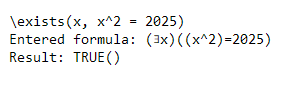
\includegraphics[width=0.99\linewidth]{пример1.PNG} \\ а)}
    \end{minipage}
    \hfill
    \begin{minipage}[ht]{0.65\linewidth}
        \center{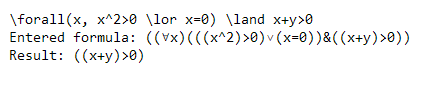
\includegraphics[width=0.99\linewidth]{пример2.PNG} \\ б)}
    \end{minipage}
    \\
    \begin{center}
        \begin{minipage}[ht]{0.8\linewidth}
            \center{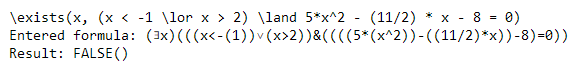
\includegraphics[width=0.99\linewidth]{пример3.PNG} \\ в)}
        \end{minipage} 
    \end{center}
    \caption{Примеры выходных данных.}  
    \label{fig:примеры}
\end{figure}

    \section*{Заключение}
	\addcontentsline{toc}{section}{Заключение}

	Таким образом, цель данной работы достигнута, все поставленные задачи решены. В работе описан языка элементарной алгебры, приведены примеры задач элементарной алгебры, достаточно подробно описан алгоритм элиминации кванторов в этом языка~--- алгоритм Тарского. По мимо этого, алгоритм был реализован в виде компьютерной программы для достаточно важного случая~--- для формул без параметров. Эта программа включает в себя систему ввода формул языка элементарной алгебры, библиотеки классов для представления объектов этого языка и собственно реализацию алгоритма Тарского.

	В заключении хочется отметить, что алгоритм Тарского далеко не самый эффективный алгоритм, но он был первым в своем роде. Именно сконструировав этот алгоритм Альфред Тарский доказал, что элементарная алгебра допускает элиминацию кванторов, хотя до этого многие годы это считалось невозможным. 
	
	Для систем компьютерного доказательства, которые в ближайшем будущем станут очень востребованными (формальная верификация компьютерных программ), алгоритм Тарского вряд ли применим из-за крайне высокой трудоемкости. Поэтому можно продолжать работу в данному направлении и изучать другие алгоритмы элиминации кванторов. А с точки зрения математики, интересен вопрос, а какие ещё языки допускают элиминацию кванторов? Поэтому автор продолжит работу в данном направлении.

    \begin{thebibliography}{99}
    \bibitem{lect1}
    Алгоритм Тарского. Лекция 1 // Лекториум. URL: https://www.lektorium.tv/lecture/31079 (дата обращения: 01.12.2019).

    \bibitem{lect2}
    Алгоритм Тарского. Лекция 2 // Лекториум. URL: https://www.lektorium.tv/lecture/31080 (дата обращения: 01.12.2019).

    \bibitem{Gibadulin1}
    Гибадулин Р. А. Алгоритм поиска вывода в Исчислении Высказываний и его программная реализация // Современные проблемы математики и информатики~: сборник научных трудов молодых ученых, аспирантов и студентов. / Яросл. гос. ун-т им. П. Г. Демидова.~--- Ярославль: ЯрГУ, 2019.~--- Вып. 19.~--- С. 28--37.

    \bibitem{DurnevML}
    Дурнев, В. Г. Элементы теории множеств и математической логики: учеб. пособие / Яросл. гос. ун-т. им. П. Г. Демидова, Ярославль, 2009~--- 412 с.

    \bibitem{Matiyasevich}
    Матиясевич, Ю. В. Алгоритм Тарского // Компьютерные инструменты в образовании.~--- 2008. ~--- № 6. ~--- С. 14.

    \bibitem{TroelsonNet}
    Троелсен, Э. Язык программирования С\# 7 и платформы .NET и .NET Core / Э. Троелсен, Ф. Джепикс; пер. с англ. и ред. Ю.Н. Артеменко. ~--- 8-е изд. ~--- М.; СПб.: Диалектика, 2020. ~--- 1328 с.

    \bibitem{Tarski}
    Tarski, A. A Decision Method for Elementary Algebra and Geometry: Prepared for Publication with the Assistance of J.C.C. McKinsey, Santa Monica, Calif.: RAND Corporation, R-109, 1951. 

\end{thebibliography}

\addcontentsline{toc}{section}{\refname}
    
    \section*{Приложение А}
	\addcontentsline{toc}{section}{Приложение А}

	Ссылка на репозиторий на GitHub~--- https://github.com/romarioGI/Coursework2k19-2k20	
\end{document}